\documentclass[11pt]{texMemo-gibbons}
\usepackage[english]{babel}
\usepackage{graphicx}
\usepackage{blindtext}
\usepackage{amsmath,amssymb,units}
\usepackage[outdir=./]{epstopdf}
\memostudent{Ty Davis}
\memocourse{ECE 3210}
\memosubject{Lab 1, Lab Basics}
\memodate{\today}
\logo{
\includegraphics[width=0.5\textwidth]{ece_horiz.pdf}}

\begin{document}
\maketitle

\section{Introduction}
\label{sec:introduction}

Look, some more text

Many times in ``real life'' experimental situations,
a full-scale formal technical report is not necessary,
nor is it effective. A brief ``Technical Memo'' is used.
This technical memorandum, sometimes called an executive
summary, is less formal than the full report. It is
not a permanent record of the work, and hence does not
include all the details and data that should be included
in a formal report. It can be a very common way of disseminating
information within an organization. In particular, it
is used to summarize the results of technical work to
non-technical colleagues. The memo should be limited
to two-pages of text, single columns, single-spaced,
with an 11-point font.  

The introduction section of the memo should cover what
the basic idea of the lab is.  It doesn't need to be
particularly long, but it should be more than a single
sentence.  

\section{Theory}
\label{sec:theory}

The theory section of the memo should cover the theory
behind the lab.  For example, if there is a derivation
needed, include that here.  When you write up a derivation,
you don't need to show every single step of mathematical
manipulation, but you need to include enough steps such
that a typical engineer could follow it.  You must typeset
your equation using the \LaTeX  equation editor to make
it look good.

For example, suppose we need to compute the complex
exponential Fourier series coefficients for a saw-tooth
waveform.  We know that $T_0=2$ and $\omega_0=\pi$.
We write out the integral we need to solve

\begin{equation}
  \label{eq:1}
  D_n = \frac{1}{2}\int^2_0 t e^{-j\pi n t} dt.  
\end{equation}

We don't need to go through and show every step of the
derivation.  It would be sufficient to say that solving
the integral yields

\begin{equation}
  \label{eq:2}
  D_n = \frac{j}{\pi n}.
\end{equation}


\section{Results}
\label{sec:results}

The results section covers the results from the lab.
Your data will mostly be represented in plots and tables.
Include those figures AFTER the main body of text on
a new page.  Data interpretation (what the plots \emph{mean})
should be reserved for the Conclusions section of the
memo.  You should comment on the trends of what you
have seen, but do not explain \emph{why} you are seeing
them in this section.

As an example, Fig.~\ref{fig:ex01} is an example of
what a proper figure should look like.  Each figure
should be properly labeled with decently sized fonts.
In the results section, you could comment  on the oscillations
in $v_2(t)$, but don't speculate why those oscillations
are there.  We can also include data in a table.  You
can see an example table in Tab.~\ref{tab:ex02}.  

\section{Discussion and Conclusions}
\label{sec:conclusions}

The conclusions section is for interpreting the data.
If you see a trend in your data, explain why you see
it in this section.  Use the theory you learned in class
in your explanation.

As a final note, you are expected to use this document
as a template for your lab submissions.  You are welcome
to upload this to overleaf to edit/compile the document.
Or you can work locally using whatever flavor of \LaTeX
compiler you prefer.  All you need to do is to upload
the document (and not the \LaTeX  source) to Canvas.

\clearpage

\begin{figure}[h!]
  \centering
  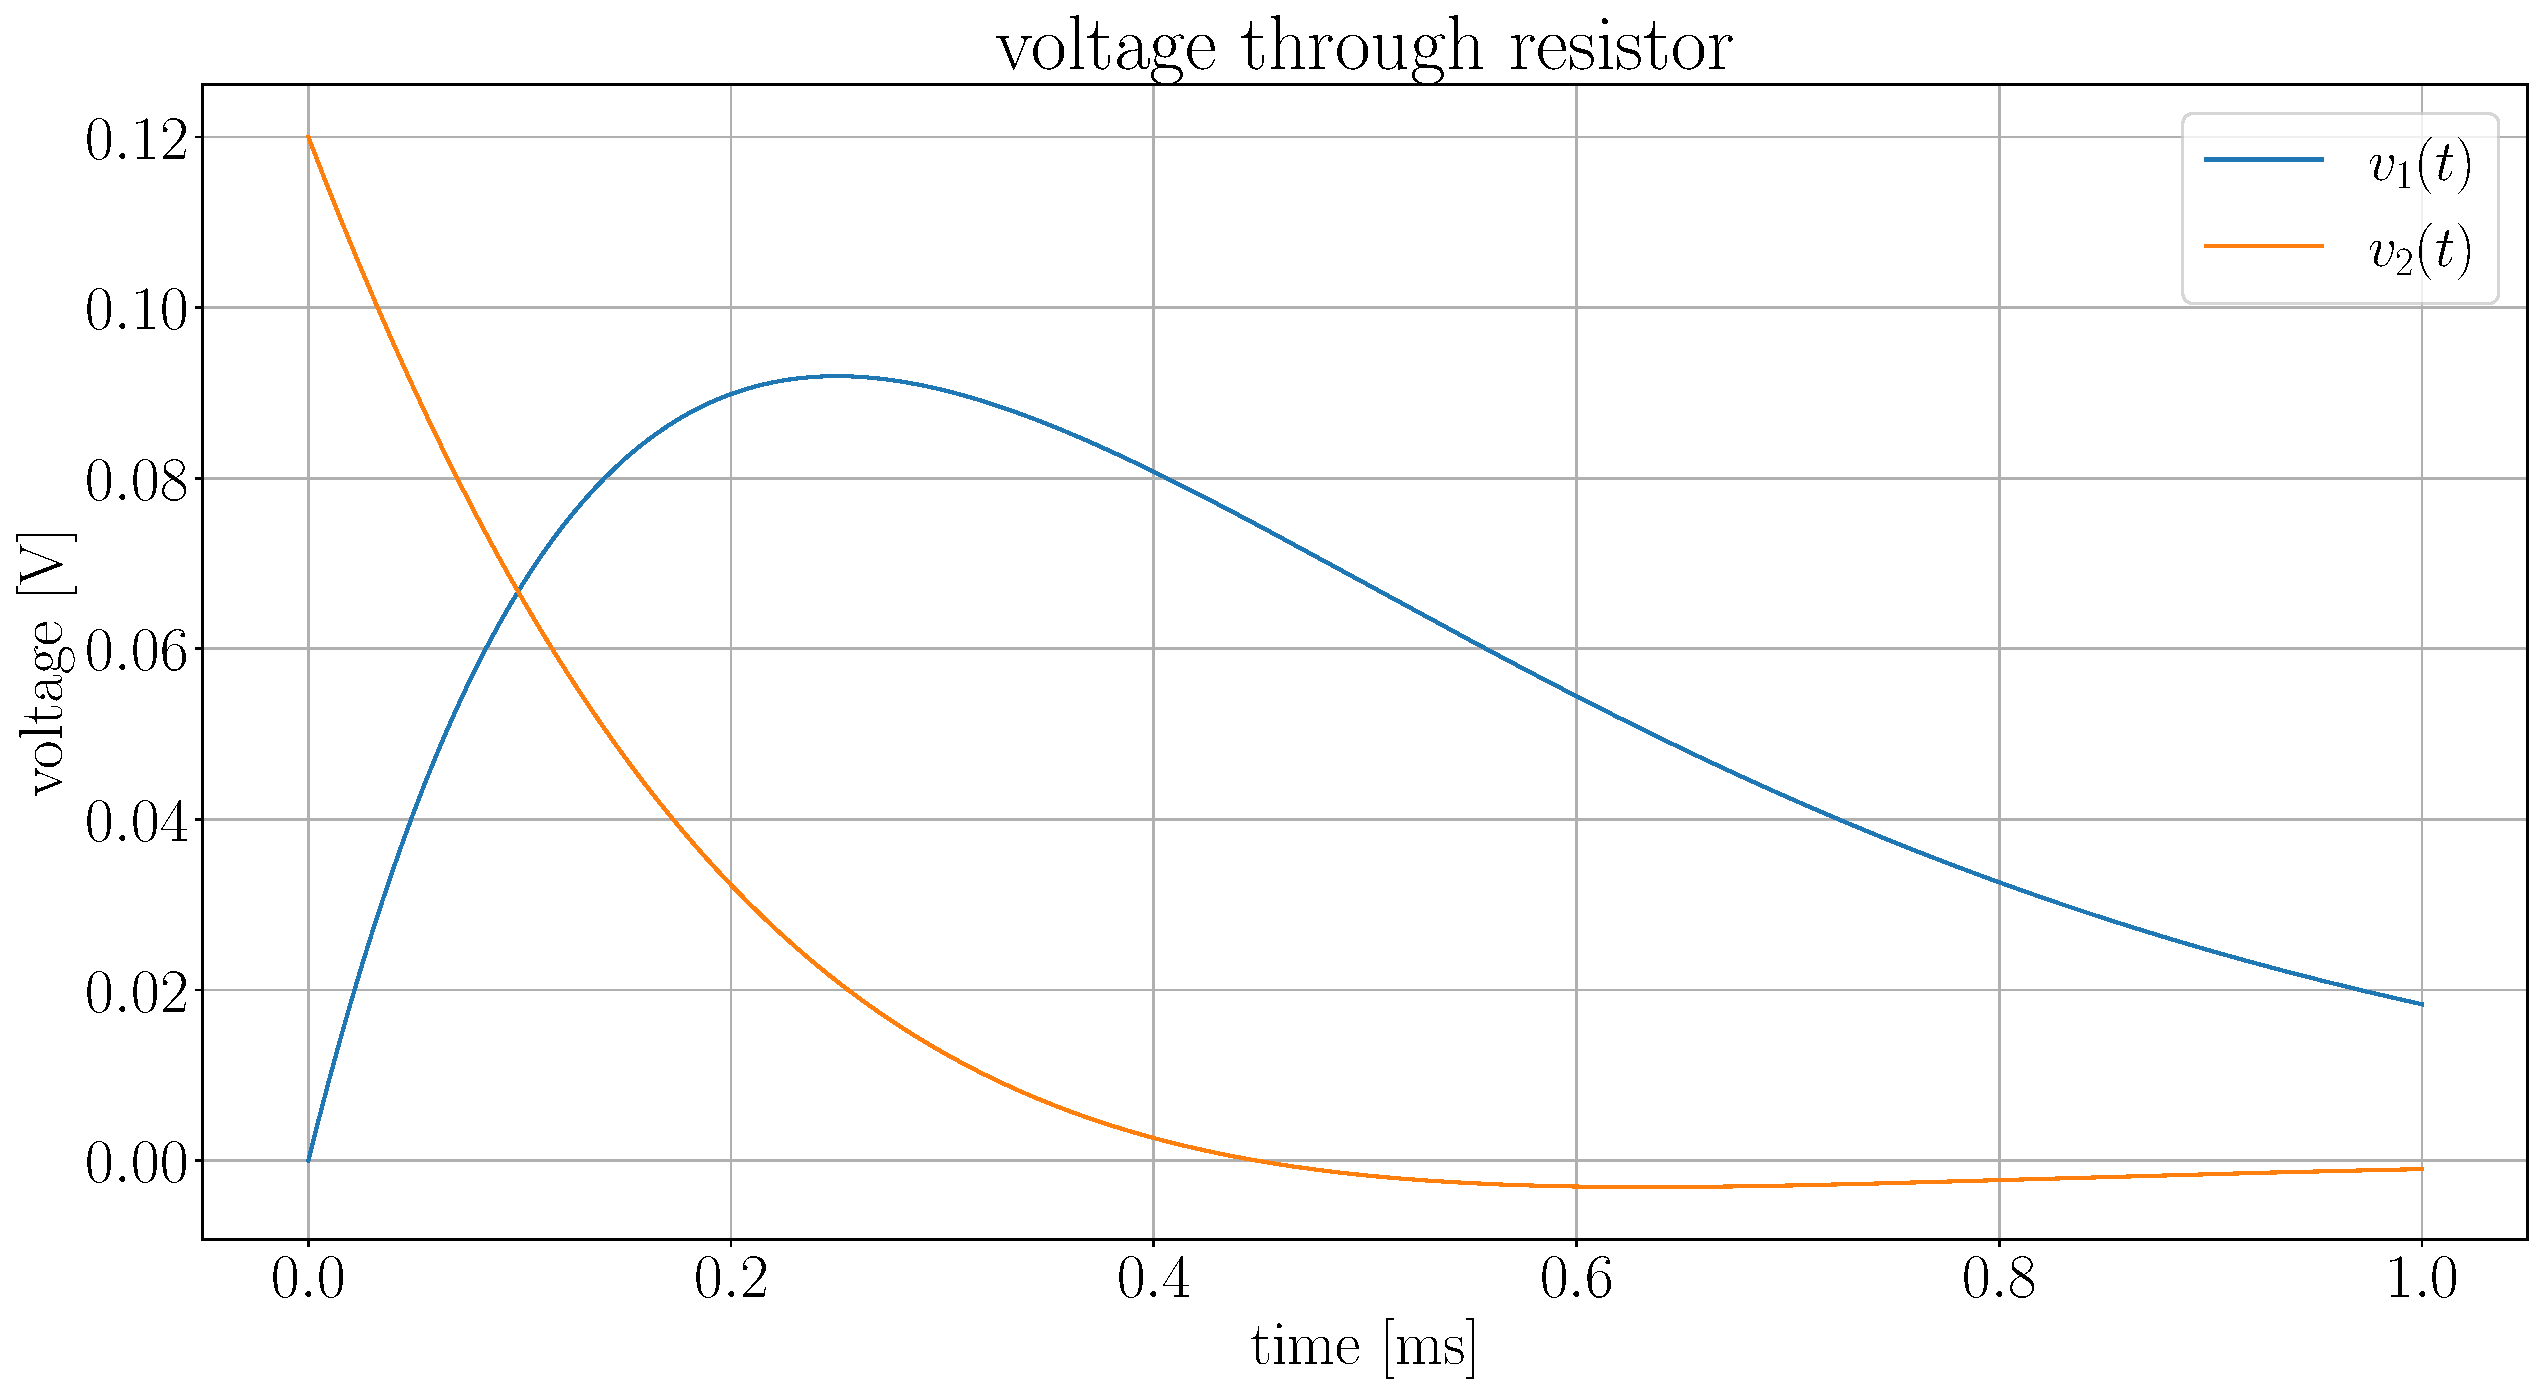
\includegraphics[width=0.7\linewidth]{fig_ex.pdf}
  \caption{every figure needs to have a detailed caption!  Most of the time people will read technical documentation and just look at the figures, so using more detail in the captions is helpful.}
  \label{fig:ex01}
\end{figure}

\begin{table}[h!]
  \centering
  \begin{tabular}{ l | c }
    \textbf{Item} & \textbf{Quantity} \\
    \hline
    $\unit[1]{k\Omega}$ resistor & 1\\
    $\unit[0.033]{\mu F}$ capacitor & 1\\
    $\unit[1]{mH}$ inductor & 1\\
  \end{tabular}
  \caption{an example of a table.  Once again, please provide a detailed description of the table in the caption.}
  \label{tab:ex02}
\end{table}



\end{document}
%%% Local Variables:
%%% mode: latex
%%% TeX-master: t
%%% End:
